\documentclass[12pt]{article}
\usepackage{amsmath, amssymb}
\usepackage{graphicx}
\usepackage{booktabs}
\usepackage{float}
\usepackage[margin=1in]{geometry}
\usepackage{setspace}
\usepackage{natbib}
\usepackage[hidelinks]{hyperref}

\begin{document}
\begin{titlepage}
    \centering
    \vspace*{3cm}
    {\Huge \textbf{Merton Jump-Diffusion: Pricing and Harvesting the Equity Jump Risk Premium} \par}
    \vspace{1.5cm}
    {\large Stochastic Processes --- Final Group Project \par}
    \vspace{2cm}
    {\Large Group 3 \par}
    \vspace{1cm}
    {\large May 5, 2026 \par}
    \vfill
\end{titlepage}

\section*{Literature Review}

The literature on asset price modelling has evolved considerably over the past five decades, moving well beyond the classical Black--Scholes framework in response to persistent empirical evidence that real financial markets are richer and more complex than any simple diffusion model can capture. This review traces that evolution across four connected areas. We begin with the foundational jump-diffusion models of Merton (1976) and Kou (2002), which introduced discontinuous price dynamics into option pricing theory, and the empirical diagnostics of Carr and Wu (2003), which confirmed that jumps are genuinely present in market data. We then turn to Eraker, Johannes, and Polson (2003), who demonstrated that both return jumps and volatility jumps are needed to fit index data, and discuss how self-exciting Hawkes processes extend this insight by allowing jump intensity to vary endogenously. Finally, we review the deep learning approach of Agram, \O{}ksendal, and Rems (2024), who address the hedging problem in incomplete jump-diffusion markets using neural network methods.

\subsection*{Classical Jump-Diffusion Processes}

The starting point for any study of discontinuous price dynamics is the Black--Scholes model, which assumes that the stock price follows a geometric Brownian motion with constant variance. While analytically tractable and elegant, the model has two well-known empirical failures. First, real return distributions exhibit leptokurtosis, with heavier tails than any normal distribution can accommodate. Second, implied volatilities extracted from observed option prices form a systematic skew or smile across strikes and maturities, rather than remaining flat as the model predicts. Both failures point in the same direction: actual price processes contain sudden, discontinuous moves that a continuous diffusion cannot generate.

Merton (1976) was the first to formally address this by adding a Poisson-driven jump process to geometric Brownian motion. He modelled the total change in the stock price as the sum of an ordinary diffusive component, representing the gradual arrival of information, and an abnormal component, representing the sudden impact of firm-specific news. Formally, the stock price dynamics are
\begin{equation}
\frac{dS}{S} = (\alpha - \lambda k)\,dt + \sigma\,dZ + dq,
\end{equation}
where $\alpha$ is the instantaneous expected return, $\sigma^2$ is the diffusive variance conditional on no jump, $dZ$ is a standard Brownian motion, $q(t)$ is an independent Poisson process with arrival rate $\lambda$, and $k \equiv E(Y-1)$ is the expected percentage price change per jump, with $Y$ denoting the random jump size multiplier. To price options under these dynamics, Merton observed that a riskless hedging portfolio cannot be constructed when jumps are present, since jump risk cannot be perfectly replicated by any portfolio of the stock and a risk-free bond. Under the special case where $Y$ is lognormally distributed, assuming that jump risk is non-systematic and therefore unpriced, this yields the Merton pricing formula
\begin{equation}
F(S,\tau) = \sum_{n=0}^{\infty} \frac{e^{-\lambda\tau}(\lambda\tau)^n}{n!}\,W\!\left(S X_n e^{-\lambda k\tau},\,\tau;\,E,\,\sigma^2,\,r\right),
\end{equation}
where $W(\cdot)$ is the standard Black--Scholes formula, $\tau$ is the time to expiration, $E$ is the exercise price, $r$ is the risk-free rate, and $X_n$ captures the cumulative jump factor conditional on $n$ jumps. Intuitively, the formula is an infinite weighted average of Black--Scholes prices, one for each possible number of jumps, with Poisson probabilities as weights, and reduces to Black--Scholes when $\lambda = 0$.

Despite its appeal, Merton's model has two notable limitations. Jump intensity $\lambda$ is constant, so the model cannot accommodate periods of elevated crash risk or jump clustering. Furthermore, normally distributed jump sizes imply symmetric tails, contradicting the well-documented finding that large negative equity returns are far more common than equally large positive returns.

Kou (2002) addressed both shortcomings by replacing the normal jump size distribution with an asymmetric double-exponential distribution. The asset price dynamics are
\begin{equation}
\frac{dS(t)}{S(t^-)} = \mu\,dt + \sigma\,dW(t) + d\!\left(\sum_{i=1}^{N(t)}(V_i - 1)\right),
\end{equation}
where $W(t)$ is a standard Brownian motion, $N(t)$ is a Poisson process with rate $\lambda$, and $\{V_i\}$ are i.i.d.\ non-negative random variables such that $Y = \log V$ has the density
\begin{equation}
f_Y(y) = p\cdot\eta_1 e^{-\eta_1 y}\mathbf{1}_{\{y\geq 0\}} + q\cdot\eta_2 e^{\eta_2 y}\mathbf{1}_{\{y < 0\}},\quad \eta_1 > 1,\; \eta_2 > 0,
\end{equation}
where $p$ and $q = 1-p$ are the probabilities of upward and downward jumps, and $1/\eta_1$ and $1/\eta_2$ are their respective mean sizes. The asymmetry between $\eta_1$ and $\eta_2$ directly captures the observation that market crashes are typically sharper than market rallies, which is particularly relevant for a technology-heavy index like the Nasdaq-100.

Beyond its empirical realism, the double-exponential distribution carries a significant mathematical advantage. Because exponential distributions are memoryless, the overshoot beyond a boundary also follows an exponential distribution and is conditionally independent of the first passage time. This structure enables closed-form solutions for path-dependent instruments --- barrier options, lookback options, and perpetual American options --- that are unavailable under Merton's normal jump specification. For European options, the pricing formula takes the form of a Poisson-weighted sum
\begin{equation}
f_n(S,\tau) = W\!\left(S,\,\tau;\,E,\,\sigma^2 + \frac{n\delta^2}{\tau},\,r\right),
\end{equation}
where $\delta^2$ is the variance of the logarithmic jump size and $f_n$ is the option price conditional on exactly $n$ jumps. Kou (2002) showed that the model reproduces the leptokurtic feature of daily returns and generates the asymmetric volatility skew observed in equity options, making it substantially more flexible than Merton's specification with a similarly parsimonious parameter set.

A limitation shared by both models is that jump intensity $\lambda$ is constant. Carr and Wu (2003) approached this problem from a different angle: rather than proposing a new parametric model, they asked whether one can determine directly from observed option prices, without committing to any specific model, whether the underlying process contains a continuous component, a jump component, or both. The key insight is that the short-maturity behaviour of out-of-the-money (OTM) options is a sensitive diagnostic of the underlying process. Under a purely continuous diffusion, OTM option prices decay at the exponentially fast rate $O(e^{-c/T})$ for some constant $c > 0$. Under any process with a jump component, a single jump can bring an OTM option into the money at any moment, so prices decay only at the much slower rate $O(T)$. Carr and Wu formalised this through a decomposition of the time value of a European option,
\begin{equation}
TV_0(K,T) = e^{-rT}\int_0^T\!\left[\tfrac{1}{2}q(K,t)K^2\,E_0\!\left[\sigma_t^2\,\big|\,F_{t^-}=K\right] + E_0\!\left[F_{t^-}\,v^0_t(k)\right]\right]dt,
\end{equation}
showing how the continuous martingale component and the jump compensator each contribute to option prices. They then proposed plotting $\ln(P/T)$ against $\ln T$ --- a term decay plot --- and reading off the slope at short maturities. A flat slope near zero for OTM options signals a jump component; a sharply negative slope signals a pure diffusion; intermediate ATM slopes distinguish finite-variation from infinite-variation jump processes.

Applying this methodology to S\&P 500 index options from April 1999 to May 2000, Carr and Wu found strong evidence for both a continuous and a jump component in index dynamics. The continuous component was persistently present throughout the sample, while the jump component varied substantially over time and was negatively correlated (around $-0.58$) with the level of implied volatility. This finding validates the general approach of Merton and Kou while simultaneously pointing to their most important limitation: they cannot accommodate the time-varying nature of jump intensity. For any empirical project working with index options, the Carr--Wu diagnostic therefore provides a model-free first check before any parametric calibration is attempted.

\subsection*{Stochastic Volatility and Jump Clustering}

While Merton and Kou represent genuine progress over Black--Scholes, both assume constant jump intensity, an assumption the evidence increasingly challenged. A natural baseline for richer dynamics is the stochastic volatility (SV) model of Heston (1993), in which the instantaneous variance $V_t$ follows a mean-reverting square-root process. Even this model falls short, as Eraker, Johannes, and Polson (2003) demonstrated through a careful likelihood-based study of S\&P 500 and Nasdaq 100 daily returns. The pure SV model still fails to generate the extreme returns observed during crises without implausibly large diffusive shocks; on the day of the October 1987 crash, it would require a return innovation of nearly eight standard deviations to produce the observed $-23\%$ move.

The natural fix is to add return jumps, giving the SVJ model. In this specification the log-price $Y_t = \log S_t$ satisfies
\begin{equation}
dY_t = \mu\,dt + \sqrt{V_{t^-}}\,dW^Y_t + \xi^Y\,dN^Y_t,
\end{equation}
where $N^Y_t$ is a Poisson process with constant intensity $\lambda^Y$ and $\xi^Y \sim N(\mu_Y, \sigma_Y^2)$ is the normally distributed jump size. The variance process evolves as
\begin{equation}
dV_t = \kappa(\theta - V_t)\,dt + \sigma_v\sqrt{V_t}\,dW^V_t,
\end{equation}
with $\mathrm{Corr}(dW^Y_t, dW^V_t) = \rho\,dt$ capturing the leverage effect. Adding return jumps reduces the estimated diffusive volatility of volatility $\sigma_v$ and the speed of mean reversion $\kappa$, and jumps account for roughly 15\% of total return variance in the SVJ model.

However, the SVJ model is itself misspecified in a revealing way. Under a constant-intensity Poisson assumption averaging roughly 1.5 arrivals per year, the SVJ algorithm identifies three separate jump arrivals during the week of the 1987 crash alone --- an implausible outcome under the model's own distributional assumptions. This clustering signals a systematic misfit: the model has no mechanism to link the occurrence of one jump to the likelihood of the next.

The solution proposed by Eraker et al.\ is to allow volatility itself to jump. In the SVCJ model --- stochastic volatility with contemporaneous jumps --- the variance equation becomes
\begin{equation}
dV_t = \kappa(\theta - V_t)\,dt + \sigma_v\sqrt{V_{t^-}}\,dW^V_t + \xi^V\,dN_t,
\end{equation}
where $N_t$ is shared with the return-jump process, $\xi^V \sim \mathrm{Exp}(\mu_V)$ ensures positive volatility jumps, and the return jump conditional on the volatility jump is $\xi^Y \mid \xi^V \sim N(\mu_Y + \rho_J\xi^V, \sigma_Y^2)$. A volatility jump provides a persistent shock to the conditional distribution of future returns, whereas a return jump is transient: it shifts today's price but leaves tomorrow's variance unaffected. In the SVCJ model, the 1987 crash week is explained by a single large contemporaneous jump driving a $-14\%$ return while simultaneously pushing annualised volatility from around 40\% to just over 50\%, after which volatility mean-reverts gradually --- a far more economically coherent story than three independent Poisson arrivals in a single week.

Estimation is carried out by Markov Chain Monte Carlo (MCMC), which recovers the full joint posterior of parameters and latent states --- spot volatility, jump times, and jump sizes --- simultaneously. Formal Bayes factors strongly favour the SVCJ specification: the log Bayes factor comparing the SV model to the SVIJ specification (independent jumps in returns and volatility) is 59.45, constituting decisive evidence in favour of the richer model by the Kass--Raftery scale. From an option-pricing perspective, volatility jumps steepen the implied volatility smile and generate the characteristic ``hook'' for in-the-money options, a feature entirely absent from the SVJ model.

Despite these improvements, the SVCJ model still assumes constant jump intensities $\lambda^Y$ and $\lambda^V$, and the authors' own diagnostics undermine this assumption: jump times cluster in crisis periods, inconsistent with a homogeneous Poisson process. Hawkes (1971) self-exciting processes provide the natural mechanism for endogenising this behaviour. In a Hawkes process, the intensity $\lambda(t)$ increases each time a jump arrives and then decays back toward a baseline level:
\begin{equation}
\lambda(t) = \mu + \int_{-\infty}^{t}\varphi(t-s)\,dN(s),
\end{equation}
where $\mu > 0$ is the background intensity and $\varphi(\cdot) \geq 0$ is the excitation kernel, typically taken to be $\varphi(u) = \alpha e^{-\beta u}$ with $\alpha < \beta$ to ensure stationarity. Each jump raises $\lambda(t)$ by $\alpha$, making the next arrival more likely; but this excess intensity decays at rate $\beta$, so the process eventually returns to $\mu$. This structure captures both the clustering of jumps during market stress and their eventual dissipation.

Gonzato and Sgarra (2021) provide a recent example of how self-exciting jumps can be used in a financial jump model. They study a specification in which the arrival of one jump increases the probability of future jumps, allowing the model to reproduce clustering during turbulent periods. Although their empirical application is to the oil market, the mechanism is directly relevant for equity index options: crashes and earnings-related shocks are rarely isolated events, and a constant Poisson intensity may underestimate the persistence of jump risk after the first shock.

Calibration typically proceeds by maximum likelihood for moderate sample sizes or Sequential Monte Carlo (SMC) when jump sizes are also stochastic and the state space becomes high-dimensional. For the present project, the Hawkes framework serves primarily as a conceptual benchmark: the Merton and Kou models, with their constant $\lambda$, sit at one extreme of the spectrum, while the Hawkes model, with fully endogenous intensity, sits at the other.

\subsection*{Machine Learning Extensions of Stochastic Processes}

Both classical jump-diffusion models and richer stochastic volatility plus jump specifications produce analytical solutions only in special cases. Once one moves to genuinely incomplete markets --- where the number of independent risk sources exceeds the number of traded assets, which is the generic situation when multiple Brownian motions or Poisson processes are present --- closed-form hedging strategies cease to exist. This is precisely the setting studied by Agram, \O{}ksendal, and Rems (2024), who propose a deep learning approach to the minimal variance (quadratic) hedging problem.

The market model considered is a single risky asset whose price $S(t)$ satisfies
\begin{equation}
dS(t) = S(t^-)\!\left[\alpha(t)\,dt + \sigma(t)\,dB(t) + \int_{\mathbb{R}^*}\!\gamma(t,\zeta)\,\tilde{N}(dt,d\zeta)\right],\quad S(0)>0,
\end{equation}
where $B(t)$ is an $m$-dimensional Brownian motion, $\tilde{N}$ is a $k$-dimensional compensated Poisson random measure, and $\alpha, \sigma, \gamma$ are deterministic and bounded. The market is incomplete when $m > 1$ or $k > 1$. For a self-financing portfolio $\pi(t)$ representing the fraction of wealth invested in the risky asset, the wealth process $X(t)$ evolves accordingly, and the hedging objective is to minimise
\begin{equation}
J(z,\pi) = E\!\left[\tfrac{1}{2}\bigl(X^{z,\pi}(T) - F\bigr)^2\right].
\end{equation}
Agram et al.\ frame this as a Stackelberg game: the first player chooses the initial endowment $z$ (the option price), and the second then selects the optimal portfolio $\hat{\pi}$ given that endowment. The main theoretical result is that the minimal variance price can be written as an expectation under a specific equivalent martingale measure $Q^*$:
\begin{equation}
\hat{z} = E^{Q^*}[F],
\end{equation}
where $Q^*$ is characterised by a Radon--Nikod\'{y}m derivative involving $G(t) = -\alpha(t)/\bigl(\sigma^2(t) + \int\gamma^2(t,\zeta)\,\nu(d\zeta)\bigr)$. Crucially, $Q^*$ is a genuine positive equivalent martingale measure rather than a signed measure, which is not guaranteed in general incomplete markets.

In more complex settings, the price integral $E^{Q^*}[F]$ and the corresponding portfolio must be computed numerically. Agram et al.\ propose a neural network algorithm combining a feed-forward layer to estimate the option price $z_0$ with a two-layer Long Short-Term Memory (LSTM) network to approximate the optimal portfolio $\pi_t$ at each time step. The LSTM architecture is well suited to this problem: the optimal portfolio is adapted to the filtration generated by the price process, so past observations are relevant for each decision, and LSTM cells maintain a memory state that allows the network to learn how past jumps affect the current hedging ratio --- especially valuable when latent volatility evolves stochastically.

The algorithm is tested on four model environments. In the Black--Scholes benchmark, it converges to the theoretical option price of 0.500 and recovers the delta hedge accurately. For the Merton jump-diffusion model, the minimal variance price is $\hat{z} = 0.519$, exceeding the Merton model's own price of 0.515. This difference arises because the Merton approach assumes jump risk is diversifiable and therefore receives no risk premium, whereas the minimal variance approach explicitly prices the unhedgeable component. The practical consequence is stark: standard Merton delta hedging produces a skewed distribution of hedging errors --- small gains most of the time but occasional large losses when a jump occurs --- whereas the minimal variance hedge yields a roughly symmetric error distribution with virtually no extreme losses. The algorithm also converges to a reasonable estimate for the Kou double-exponential model, where no closed-form equivalent martingale measure price exists.

The main limitations concern scalability and interpretability: convergence slows after a few thousand training epochs, training time grows substantially with the number of time-discretisation steps, and accuracy decreases as option maturity lengthens due to accumulating discretisation errors. Despite these drawbacks, the framework represents a genuine advance over purely analytical methods because it handles models --- such as the Kou model with two-sided jumps, or future extensions incorporating stochastic volatility and self-exciting jump intensity --- where closed-form solutions simply do not exist.

\subsection*{Research Frontier and Connection to Our Project}

Taken together, the literature reviewed above traces a coherent arc from the first principled treatment of jump risk through to the modern machine learning frontier. Merton (1976) broke with the continuity assumption of Black--Scholes and provided the first tractable framework for option pricing under jump risk. Kou (2002) extended this by replacing the symmetric normal jump distribution with an asymmetric double-exponential, capturing the empirical reality that crashes are sharper than rallies and enabling closed-form solutions for a wider class of options. Carr and Wu (2003) confirmed empirically that both continuous and jump components are present in S\&P 500 index options, and that their relative importance varies systematically over time. Eraker, Johannes, and Polson (2003) demonstrated through Bayesian estimation that stochastic volatility alone is insufficient and that both return and volatility jumps are necessary to fit index data. The Hawkes framework provides one natural way to endogenise jump clustering, while the deep learning approach of Agram et al.\ (2024) addresses the pricing and hedging problem in incomplete markets where analytical solutions are unavailable.

Several unresolved tensions emerge from this literature. The most fundamental is the trade-off between empirical richness and analytical tractability. The Merton and Kou models are estimable but too restrictive, unable to accommodate time-varying jump intensity or persistent volatility jumps. The SVCJ model fits the data better but requires computationally intensive MCMC estimation. The Hawkes framework adds endogenous clustering but raises its own estimation challenges and has not been as thoroughly tested against option-implied data as the parametric jump-diffusion models. The deep learning approach of Agram et al.\ is the most flexible but sacrifices interpretability.

A second tension concerns the identification of jump risk premia. Both Merton and Kou price options without explicitly modelling the compensation that investors require for bearing jump risk. The finding that the minimal variance price exceeds the Merton price aligns with the expectation that implied volatilities should be systematically above the levels implied by the physical measure. For a technology index like the Nasdaq-100, where sector-specific crashes can be swift and severe, this premium is likely to be economically significant and is one of the central quantities of interest in the present project.

A third consideration is the diagnostic value of the Carr--Wu term decay methodology. Before committing to any parametric model, plotting term decay curves for short-maturity options will indicate whether a finite-variation jump component of the Merton or Kou type is sufficient, or whether the data hints at infinite-variation or time-varying intensity dynamics. A flat OTM slope near zero at short maturities would confirm a Poisson-type jump component, while a clearly negative slope would point toward infinite-variation L\'{e}vy components or stochastic volatility extensions.

Looking forward, the literature suggests several natural extensions. One is to replace the constant Poisson intensity in the Merton and Kou models with a Hawkes self-exciting intensity, capturing jump clustering during stress periods without the full computational burden of MCMC. Another is to apply the LSTM-based hedging algorithm of Agram et al.\ to produce out-of-sample hedging strategies for QQQ options that are more robust to jump risk than standard delta hedging. A third is to estimate the models jointly from time-series returns and option prices to obtain internally consistent estimates of both the physical and risk-neutral jump parameters. Each extension would move the analysis closer to the frontier of what the recent literature has demonstrated is both theoretically justified and empirically important.

\paragraph{Literature Review Summary.}
The literature reviewed in this chapter documents a clear progression in the understanding and modelling of discontinuous price dynamics. Black--Scholes fails on two empirically important counts: it cannot generate the heavy tails and negative skewness of real return distributions, and it produces a flat implied volatility surface rather than the skew or smile that options markets consistently display. Merton (1976) introduced a Poisson-driven jump process alongside the diffusion and derived an option pricing formula that nests Black--Scholes as a special case, but relies on symmetric normal jump sizes and a constant arrival rate. Kou (2002) improved on the first assumption by replacing the normal distribution with an asymmetric double-exponential, while both models leave jump intensity constant. Carr and Wu (2003) confirmed empirically that jumps are present in index options data and that their importance varies over time. Eraker, Johannes, and Polson (2003) showed through Bayesian estimation that stochastic volatility alone is insufficient, and that contemporaneous jumps in both returns and volatility are decisively preferred by the data. Hawkes processes extend this insight by formalising the endogenous clustering of jumps during market stress. Finally, the deep learning framework of Agram et al.\ (2024) provides a formal confirmation that jump risk commands a positive premium in incomplete markets, and that ignoring it leads to systematically biased hedges and unexpected losses.

No single model explains financial markets perfectly: each involves a compromise between empirical fit, analytical tractability, and estimation feasibility. This honest recognition of limitations is precisely what motivates continued research into stochastic jump-diffusion processes and makes the study of jump risk premia in real option markets --- the focus of the present project --- both timely and relevant.

\newpage
\section*{Mathematical Derivations}
\label{sec:mathematical_derivations}

This section fixes the mathematical notation used in the pricing, Monte Carlo, COS, calibration, and hedging parts of the project. We focus on the Merton jump-diffusion model as the main model and on the Kou double-exponential jump model as the benchmark extension. The goal is not only to state the formulas, but to show why the drift correction, characteristic functions, and incompleteness results arise naturally.

\subsection*{Physical and Risk-Neutral Dynamics}

Let $(\Omega,\mathcal{F},(\mathcal{F}_t)_{t\geq 0},\mathbb{P})$ be a filtered probability space supporting a Brownian motion $W_t^{\mathbb{P}}$ and a Poisson process $N_t^{\mathbb{P}}$ with intensity $\lambda^{\mathbb{P}}$. The jump sizes are represented by i.i.d. random variables $J_i$, independent of both $W^{\mathbb{P}}$ and $N^{\mathbb{P}}$. If $Y_i=e^{J_i}$ denotes the gross jump multiplier, then a jump changes the stock price from $S_{t^-}$ to $S_t=S_{t^-}Y_i$.

Under the physical measure $\mathbb{P}$, the model can be written as
\begin{equation}
\frac{dS_t}{S_{t^-}}
= \left(\mu - \lambda^{\mathbb{P}}\kappa^{\mathbb{P}}\right)dt
+ \sigma dW_t^{\mathbb{P}}
+ (e^{J}-1)dN_t^{\mathbb{P}},
\label{eq:p_dynamics}
\end{equation}
where
\begin{equation}
\kappa^{\mathbb{P}} = \mathbb{E}^{\mathbb{P}}[e^J-1]
\label{eq:kappa_p}
\end{equation}
is the expected percentage jump size under $\mathbb{P}$. The physical parameters describe the historical behaviour of returns and will later be estimated from high-frequency QQQ data and jump detection tests.

For pricing, we work under a risk-neutral measure $\mathbb{Q}$. The discounted stock price must be a martingale under $\mathbb{Q}$, so the drift is replaced by the risk-free rate and corrected for the expected jump contribution. The risk-neutral dynamics are
\begin{equation}
\frac{dS_t}{S_{t^-}}
= \left(r - \lambda^{\mathbb{Q}}\kappa^{\mathbb{Q}}\right)dt
+ \sigma dW_t^{\mathbb{Q}}
+ (e^{J}-1)dN_t^{\mathbb{Q}},
\label{eq:q_dynamics_general}
\end{equation}
where
\begin{equation}
\kappa^{\mathbb{Q}} = \mathbb{E}^{\mathbb{Q}}[e^J-1].
\label{eq:kappa_q}
\end{equation}
In the rest of this section we suppress the superscript $\mathbb{Q}$ and write $\lambda$ and $\kappa$ for risk-neutral quantities. The difference between the physical jump intensity $\lambda^{\mathbb{P}}$ and the calibrated risk-neutral intensity $\lambda^{\mathbb{Q}}$ is economically important: it is one way to measure the jump risk premium.

\subsection*{Change of Measure and Girsanov Argument}

Before deriving the Merton stock-price dynamics, we briefly clarify how the passage from the physical measure $\mathbb{P}$ to the pricing measure $\mathbb{Q}$ is represented in our notation. The passage from $\mathbb{P}$ to $\mathbb{Q}$ can be viewed as a change of measure. For the Brownian part, Girsanov's theorem changes only the drift. In the simple constant-coefficient case, define
\begin{equation}
\frac{d\mathbb{Q}}{d\mathbb{P}}\bigg|_{\mathcal{F}_T}
=\exp\left(-\theta W_T^{\mathbb{P}}-\frac{1}{2}\theta^2T\right),
\qquad
W_t^{\mathbb{Q}}=W_t^{\mathbb{P}}+\theta t.
\label{eq:girsanov_density}
\end{equation}
Then $W_t^{\mathbb{Q}}$ is a Brownian motion under $\mathbb{Q}$, and the Brownian drift can be adjusted so that the discounted stock price is a martingale. In a pure diffusion model this would pin down the unique risk-neutral measure. In a jump-diffusion model, however, the jump intensity and jump-size distribution may also change under the pricing measure. Since jump risk is not perfectly hedgeable, no-arbitrage does not determine this jump-risk adjustment uniquely. For this reason, our empirical implementation estimates physical jump parameters from returns but calibrates risk-neutral jump parameters directly from option prices. This is the practical link between Girsanov's theorem, market incompleteness, and the jump risk premium discussed in this project \citep{Shreve2004}.

\subsection*{From the Log-Price to the Stock-Price SDE}

Define the log-price process
\begin{equation}
X_t=\log S_t.
\label{eq:log_price}
\end{equation}
For a finite-activity jump-diffusion, the risk-neutral log-price dynamics are
\begin{equation}
dX_t=
\left(r-\lambda\kappa-\frac{1}{2}\sigma^2\right)dt
+\sigma dW_t^{\mathbb{Q}}+JdN_t.
\label{eq:log_sde}
\end{equation}
The term $-\frac{1}{2}\sigma^2$ is the usual It\^{o} correction from geometric Brownian motion, while $-\lambda\kappa$ compensates for the average jump growth.

To recover the stock-price dynamics, apply It\^{o}'s formula for jump processes to $S_t=e^{X_t}$. Between jumps, the continuous part gives
\begin{equation}
\frac{dS_t}{S_t}=
\left(r-\lambda\kappa\right)dt+\sigma dW_t^{\mathbb{Q}}.
\end{equation}
At a jump time, $\Delta X_t=J$, hence
\begin{equation}
\Delta S_t=S_{t^-}(e^J-1).
\end{equation}
Combining the continuous and jump parts gives exactly
\begin{equation}
\frac{dS_t}{S_{t^-}}=
(r-\lambda\kappa)dt+\sigma dW_t^{\mathbb{Q}}+(e^J-1)dN_t,
\label{eq:merton_sde_final}
\end{equation}
which is the Merton jump-diffusion SDE used throughout the project.

\subsection*{Martingale Condition}

The risk-neutral drift in Equation~\eqref{eq:merton_sde_final} is chosen so that the discounted price $e^{-rt}S_t$ is a $\mathbb{Q}$-martingale. Let $\tau=T-t$. Solving Equation~\eqref{eq:log_sde} over $[t,T]$ gives
\begin{equation}
S_T=S_t\exp\left[
\left(r-\lambda\kappa-\frac{1}{2}\sigma^2\right)\tau
+\sigma(W_T^{\mathbb{Q}}-W_t^{\mathbb{Q}})
+\sum_{i=1}^{N_\tau}J_i
\right].
\label{eq:st_solution}
\end{equation}
Since the Brownian and jump parts are independent,
\begin{align}
\mathbb{E}_t^{\mathbb{Q}}[S_T]
&=S_t e^{(r-\lambda\kappa-\frac12\sigma^2)\tau}
\mathbb{E}^{\mathbb{Q}}\!\left[e^{\sigma(W_T-W_t)}\right]
\mathbb{E}^{\mathbb{Q}}\!\left[e^{\sum_{i=1}^{N_\tau}J_i}\right].
\end{align}
The Brownian expectation is
\begin{equation}
\mathbb{E}^{\mathbb{Q}}\!\left[e^{\sigma(W_T-W_t)}\right]
=e^{\frac12\sigma^2\tau},
\end{equation}
and the compound Poisson expectation is
\begin{equation}
\mathbb{E}^{\mathbb{Q}}\!\left[e^{\sum_{i=1}^{N_\tau}J_i}\right]
=\exp\left(\lambda\tau\bigl(\mathbb{E}^{\mathbb{Q}}[e^J]-1\bigr)\right)
=e^{\lambda\kappa\tau}.
\end{equation}
Therefore,
\begin{equation}
\mathbb{E}_t^{\mathbb{Q}}[S_T]=S_t e^{r\tau},
\end{equation}
and hence
\begin{equation}
\mathbb{E}_t^{\mathbb{Q}}\left[e^{-r(T-t)}S_T\right]=S_t.
\label{eq:martingale_result}
\end{equation}
Thus the discounted stock price is a martingale under $\mathbb{Q}$, which is the no-arbitrage condition needed for risk-neutral valuation.

\subsection*{Characteristic Function of the Merton Model}

Fourier and COS pricing methods require the characteristic function of $X_T=\log S_T$. From Equation~\eqref{eq:st_solution}, for any real $u$,
\begin{equation}
\begin{aligned}
\phi_X(u;t,T)
&= \mathbb{E}_t^{\mathbb{Q}}\!\left[e^{iuX_T}\right] \\
&= \exp\!\Bigg(
iu\Big[x_t+\Big(r-\lambda\kappa-\tfrac12\sigma^2\Big)\tau\Big]
-\tfrac12\sigma^2u^2\tau \\
&\qquad\qquad
+\lambda\tau\big(\Psi_J(u)-1\big)
\Bigg).
\end{aligned}
\label{eq:general_cf}
\end{equation}
where
\begin{equation}
\Psi_J(u)=\mathbb{E}^{\mathbb{Q}}[e^{iuJ}]
\label{eq:jump_cf}
\end{equation}
is the characteristic function of the log-jump size.

In the Merton model,
\begin{equation}
J\sim N(\mu_J,\sigma_J^2).
\end{equation}
Therefore,
\begin{equation}
\Psi_J(u)=\exp\left(iu\mu_J-\frac12u^2\sigma_J^2\right),
\label{eq:merton_jump_cf}
\end{equation}
and
\begin{equation}
\kappa=\mathbb{E}[e^J-1]
=\exp\left(\mu_J+\frac12\sigma_J^2\right)-1.
\label{eq:merton_kappa}
\end{equation}
Substituting Equations~\eqref{eq:merton_jump_cf} and~\eqref{eq:merton_kappa} into Equation~\eqref{eq:general_cf} gives the Merton characteristic function used in our COS engine.

\subsection*{Merton Pricing Formula}

For a European call option with payoff $(S_T-K)^+$, the risk-neutral price is
\begin{equation}
C(t,S_t)=e^{-r\tau}\mathbb{E}_t^{\mathbb{Q}}[(S_T-K)^+].
\label{eq:risk_neutral_call}
\end{equation}
The key step is to condition on the number of jumps. Since $N_\tau\sim \mathrm{Poisson}(\lambda\tau)$,
\begin{equation}
C(t,S_t)=\sum_{n=0}^{\infty}\mathbb{P}(N_\tau=n)\,
 e^{-r\tau}\mathbb{E}_t^{\mathbb{Q}}[(S_T-K)^+\mid N_\tau=n].
\label{eq:condition_on_n}
\end{equation}
Conditional on $N_\tau=n$, the sum of log-jumps is normal:
\begin{equation}
\sum_{i=1}^{n}J_i\sim N(n\mu_J,n\sigma_J^2).
\end{equation}
Thus, conditional on $n$ jumps, the terminal log-price is still normally distributed. It can be represented as a Black--Scholes log-price with adjusted volatility
\begin{equation}
\sigma_n^2=\sigma^2+\frac{n\sigma_J^2}{\tau},
\label{eq:sigma_n}
\end{equation}
and adjusted drift parameter
\begin{equation}
r_n=r-\lambda\kappa+\frac{n\mu_J}{\tau}+\frac{n\sigma_J^2}{2\tau}.
\label{eq:r_n}
\end{equation}
The conditional Black--Scholes representation is discounted at $r_n$, while the original risk-neutral payoff in Equation~\eqref{eq:risk_neutral_call} is discounted at $r$. Therefore the conditional price contributes an additional factor $e^{(r_n-r)\tau}$. Using Equation~\eqref{eq:r_n},
\begin{equation}
e^{(r_n-r)\tau}
=\exp\left(-\lambda\kappa\tau+n\mu_J+\frac12n\sigma_J^2\right)
=e^{-\lambda\kappa\tau}(1+\kappa)^n,
\label{eq:rn_adjustment}
\end{equation}
because $1+\kappa=\exp(\mu_J+\frac12\sigma_J^2)$. Hence
\begin{equation}
e^{-\lambda\tau}\frac{(\lambda\tau)^n}{n!}e^{(r_n-r)\tau}
=
e^{-\lambda(1+\kappa)\tau}
\frac{(\lambda(1+\kappa)\tau)^n}{n!}.
\label{eq:lambda_prime_derivation}
\end{equation}
Defining $\lambda'=\lambda(1+\kappa)$, the Merton price becomes
\begin{equation}
C^{\mathrm{Merton}}(S,K,\tau)
=\sum_{n=0}^{\infty}
e^{-\lambda'\tau}\frac{(\lambda'\tau)^n}{n!}
C^{\mathrm{BS}}(S,K,\tau,r_n,\sigma_n),
\label{eq:merton_price_formula}
\end{equation}
where
\begin{equation}
\lambda'=\lambda(1+\kappa)=\lambda\exp\left(\mu_J+\frac12\sigma_J^2\right).
\label{eq:lambda_prime}
\end{equation}
This formula is useful twice in our project. First, it provides a fast semi-closed-form benchmark for European option prices. Second, it will be used as a control variate and validation target for the Monte Carlo and COS implementations.



\newpage
\section*{Monte Carlo Pricing and Validation}
\label{sec:monte_carlo}

This section describes the Monte Carlo engine used to price European options under the Merton jump-diffusion model, following standard Monte Carlo principles used in financial engineering \citep{Glasserman2004}. The implementation is designed to be consistent with the risk-neutral dynamics derived in Section~\ref{sec:mathematical_derivations}, and the analytic Merton price in Equation~\eqref{eq:merton_price_formula} is used as the validation benchmark. The goal of this workstream is not only to simulate prices, but also to test convergence, compare variance-reduction methods, and generate reproducible numerical outputs for later calibration and hedging sections.

\subsection*{Risk-Neutral Simulation Scheme}

Under the risk-neutral Merton model, the log-price satisfies
\begin{equation}
X_T = X_0 + \left(r-\lambda\kappa-\frac12\sigma^2\right)T
+\sigma W_T + \sum_{i=1}^{N_T}J_i,
\label{eq:w3_terminal_logprice}
\end{equation}
where $N_T\sim \mathrm{Poisson}(\lambda T)$ and $J_i\sim N(\mu_J,\sigma_J^2)$. In the Monte Carlo code, the original jump intensity $\lambda$ is used for path simulation. The transformed intensity $\lambda'=\lambda(1+\kappa)$ appears only in the analytic Poisson-weighted Black--Scholes formula after the algebraic rearrangement shown in Equation~\eqref{eq:lambda_prime_derivation}. This distinction is important because the simulation follows the actual jump-count process, while the analytic formula rewrites the conditional pricing mixture.

For a European call option, each simulated terminal price produces the discounted payoff
\begin{equation}
\widehat{C}_m=e^{-rT}(S_T^{(m)}-K)^+,
\end{equation}
and the plain Monte Carlo estimator is
\begin{equation}
\widehat{C}_{MC}=\frac1M\sum_{m=1}^{M}\widehat{C}_m,
\qquad
\widehat{SE}=\frac{s(\widehat{C}_1,\ldots,\widehat{C}_M)}{\sqrt{M}},
\label{eq:w3_plain_mc}
\end{equation}
where $M$ is the number of simulated paths and $s(\cdot)$ is the sample standard deviation of discounted payoffs.

The implementation supports two equivalent simulation modes. For European payoffs, the terminal representation in Equation~\eqref{eq:w3_terminal_logprice} can be sampled directly in one step. For diagnostic purposes, the code also supports a time-grid version that simulates Brownian increments and Poisson jump arrivals over $N$ time steps. Since the log-price increments are sampled exactly over each interval, the time-grid experiment should be interpreted as a numerical stability check rather than as an Euler discretisation convergence study.

\subsection*{Variance Reduction Methods}

Three variance-reduction methods are implemented and compared against the plain Monte Carlo estimator. First, antithetic variates are used for the Brownian component. For each standard normal shock $Z$, the simulation also constructs a paired path using $-Z$. The jump component is drawn independently across the two paired branches. This keeps the negative correlation generated by the diffusion part, while avoiding an artificial coupling of jump arrivals across the antithetic pair.

Second, moment matching rescales the simulated terminal prices so that their sample mean matches the martingale target $S_0e^{rT}$ implied by Equation~\eqref{eq:martingale_result}. This finite-sample correction enforces the no-arbitrage mean condition on each simulation batch and reduces bias in the estimated terminal distribution, although it does not necessarily reduce the variance of the payoff estimator.

Third, a Black--Scholes control variate is used. Let $Y$ be the discounted Merton payoff and let $X$ be the discounted Black--Scholes payoff generated from the same Brownian shocks but with jumps removed. Since the exact Black--Scholes price $C^{BS}$ is known, the control-variate estimator is
\begin{equation}
\widehat{C}_{CV}=\overline{Y}-\widehat{\beta}(\overline{X}-C^{BS}),
\qquad
\widehat{\beta}=\frac{\widehat{\mathrm{Cov}}(Y,X)}{\widehat{\mathrm{Var}}(X)}.
\label{eq:w3_control_variate}
\end{equation}
Using the same Brownian shocks is essential: it creates a strong correlation between the Merton payoff and the control payoff, which is what makes the control variate effective. The jump component remains unhedged in the control, so the method reduces variance but does not remove jump risk.

\subsection*{Control-Variate Sensitivity Study}

The effectiveness of the Black--Scholes control variate depends on how much of the Merton payoff variance comes from the diffusion component rather than from the jump component. To make this trade-off explicit, the implementation includes a sensitivity experiment that varies the jump-size volatility $\sigma_J$ while keeping the other parameters fixed. When $\sigma_J$ is small, the diffusion part explains most of the payoff variation and the control variate is more effective. As $\sigma_J$ increases, residual jump risk becomes more important and the variance reduction from the Black--Scholes control becomes weaker. The results are saved in \texttt{control\_variate\_sensitivity.csv} and visualised in \texttt{control\_variate\_sensitivity.pdf}.

\subsection*{Validation Against the Analytic Merton Price}

The exact Merton price in Equation~\eqref{eq:merton_price_formula} is used as the benchmark for validating the Monte Carlo engine. For each experiment, the absolute error is computed as
\begin{equation}
\mathrm{Error}=\left|\widehat{C}_{MC}-C^{\mathrm{Merton}}\right|.
\label{eq:w3_mc_error}
\end{equation}
The validation routine reports Monte Carlo price, standard error, exact price, absolute error, and confidence intervals. A correct implementation should show that the error decreases at the usual Monte Carlo rate $O(M^{-1/2})$ as the number of paths increases.

The code also produces a variance-reduction table comparing the plain estimator, antithetic variates, moment matching, and the Black--Scholes control variate. The main quantity of interest is the standard error. A successful variance-reduction method should reduce the standard error while keeping the estimate close to the analytic Merton benchmark.

\subsection*{Convergence and Stability Experiments}

Two numerical diagnostics are included. The path convergence experiment fixes the model parameters and increases the number of simulated paths. The expected behaviour is
\begin{equation}
\mathrm{RMSE}(M)\propto M^{-1/2},
\end{equation}
which is the standard Monte Carlo convergence rate. This experiment checks whether the empirical pricing error behaves consistently with the theory.

The time-grid stability experiment fixes the number of paths and changes the number of time steps. For a European payoff under the constant-parameter Merton model, the terminal distribution can be sampled exactly, so there should not be a meaningful discretisation bias. The purpose of this experiment is therefore to confirm that the time-stepping implementation is stable and agrees with the direct terminal simulation.

\subsection*{Implied Volatility Smile}

To connect the Monte Carlo engine to option-market diagnostics, the code computes Black--Scholes implied volatilities from Merton prices across a grid of strikes. This produces an implied volatility smile, which can be compared to the flat volatility generated by the Black--Scholes benchmark. The jump parameters have an intuitive effect: $\lambda$ increases the amount of priced tail risk, $\mu_J<0$ generates downside skew, and $\sigma_J$ increases tail thickness.

The smile experiment is important for the later calibration workstream. If the Merton model is correctly implemented, it should generate a non-flat implied volatility curve even when the diffusion volatility $\sigma$ is constant. This is the numerical counterpart of the theoretical motivation from the literature review: jumps help explain the volatility smile that Black--Scholes cannot produce.

\subsection*{Implementation and Reproducibility}

The W3 code is organised as a small reproducible pipeline rather than as a single notebook. The implementation is split into modules: configuration and environment parsing, analytical pricing, path simulation, experiments, plotting, and the main entry point. The pipeline uses fixed random seeds, command-line arguments, environment variables, logging, and CSV/PDF outputs so that results can be reviewed and reproduced on GitHub.

\begin{center}
\begin{tabular}{p{3.2cm}p{10.5cm}}
\toprule
Module & Role in the W3 pipeline \\
\midrule
\texttt{config.py} & Loads model parameters, Monte Carlo settings, command-line arguments, and environment variables. \\
\texttt{pricing.py} & Implements Black--Scholes pricing, implied volatility inversion, and the exact Merton pricing formula. \\
\texttt{simulation.py} & Simulates Merton terminal prices and time-stepped paths with variance-reduction options. \\
\texttt{experiments.py} & Runs validation, convergence, stability, smile, and variance-reduction experiments. \\
\texttt{plots.py} & Saves convergence, smile, and control-variate diagnostic figures. \\
\texttt{merton\_mc.py} & Orchestrates the full W3 pipeline and writes all outputs. \\
\bottomrule
\end{tabular}
\end{center}

The main generated outputs are listed below. These files are not hard-coded into the model itself; they are written to the configured output directory so that the same code can be rerun with different experiment settings.

\begin{center}
\begin{tabular}{p{5.0cm}p{8.8cm}}
\toprule
Output file & Purpose \\
\midrule
\texttt{validation\_summary.csv} & Compares Monte Carlo estimates with the exact Merton benchmark. \\
\texttt{variance\_reduction\_table.csv} & Reports standard errors and errors for plain MC and variance-reduced estimators. \\
\texttt{path\_convergence.csv} & Stores pricing errors for different numbers of simulated paths. \\
\texttt{time\_grid\_stability.csv} & Checks stability across different time grids. \\
\texttt{implied\_vol\_smile.csv} & Stores strike-by-strike Merton prices and implied volatilities. \\
\texttt{control\_variate\_sensitivity.csv} & Reports standard errors of the plain and control-variate estimators across different jump-volatility values. \\
\texttt{convergence\_study.pdf} & Visualises Monte Carlo convergence and time-grid stability. \\
\texttt{implied\_vol\_smile.pdf} & Visualises the Merton implied-volatility smile against the Black--Scholes benchmark. \\
\texttt{control\_variate\_sensitivity.pdf} & Visualises how control-variate efficiency changes as jump-size dispersion $\sigma_J$ increases. \\
\bottomrule
\end{tabular}
\end{center}

\IfFileExists{results/convergence_study.pdf}{%
\begin{figure}[H]
\centering
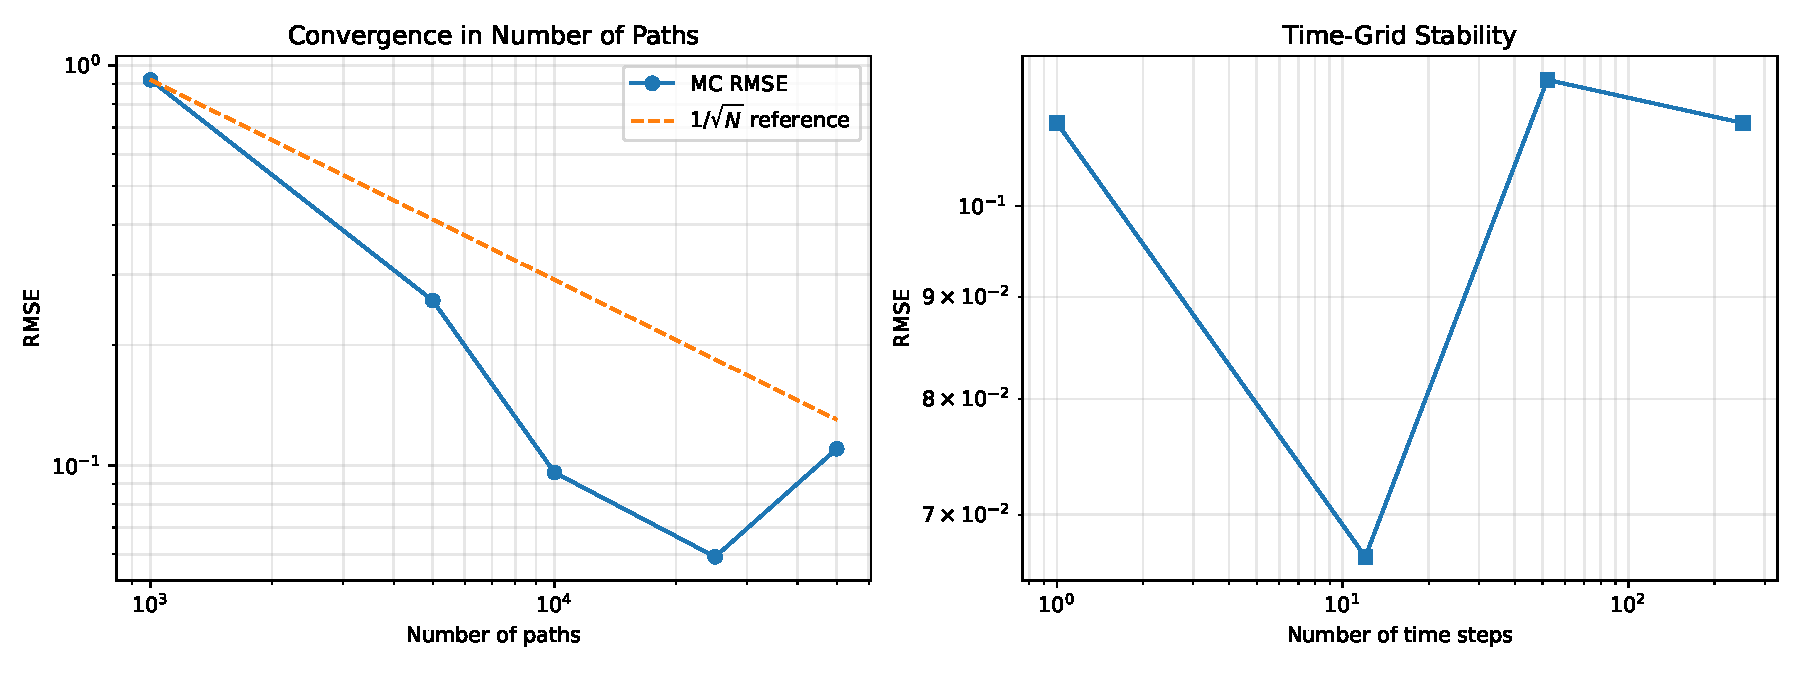
\includegraphics[width=0.88\textwidth]{results/convergence_study.pdf}
\caption{Monte Carlo path convergence and time-grid stability diagnostics generated by the W3 pipeline.}
\label{fig:w3_convergence}
\end{figure}
}{%
\noindent\textit{Note: the convergence figure is generated by running the W3 pipeline and is expected at \texttt{results/convergence\_study.pdf}.}
}

\IfFileExists{results/implied_vol_smile.pdf}{%
\begin{figure}[H]
\centering

\includegraphics[width=0.88\textwidth]{results/implied_vol_smile.pdf}
\caption{Model-implied volatility smile produced by the Merton jump-diffusion engine.}
\label{fig:w3_smile}
\end{figure}
}{%
\noindent\textit{Note: the implied-volatility smile figure is generated by running the W3 pipeline and is expected at \texttt{results/implied\_vol\_smile.pdf}.}
}

\IfFileExists{results/control_variate_sensitivity.pdf}{%
\begin{figure}[H]
\centering

\includegraphics[width=0.88\textwidth]{results/control_variate_sensitivity.pdf}
\caption{Sensitivity of the Black--Scholes control variate to jump-size volatility.}
\label{fig:w3_cv_sensitivity}
\end{figure}
}{%
\noindent\textit{Note: the control-variate sensitivity figure is generated by running the W3 pipeline and is expected at \texttt{results/control\_variate\_sensitivity.pdf}.}
}

Overall, the Monte Carlo engine validates the mathematical formulas derived in W2 and provides a numerical foundation for the later COS, calibration, and hedging workstreams. The exact Merton price is used as a benchmark, the simulation uses the same risk-neutral drift correction as the theory section, and the variance-reduction experiments make the numerical estimator more efficient and easier to validate.


\begin{thebibliography}{99}

\bibitem[Merton(1976)]{Merton1976}
Merton, R. C. (1976).
Option pricing when underlying stock returns are discontinuous.
\textit{Journal of Financial Economics}, 3(1--2), 125--144.

\bibitem[Kou(2002)]{Kou2002}
Kou, S. G. (2002).
A jump-diffusion model for option pricing.
\textit{Management Science}, 48(8), 1086--1101.

\bibitem[Carr and Wu(2003)]{CarrWu2003}
Carr, P., \& Wu, L. (2003).
What type of process underlies options? A simple robust test.
\textit{Journal of Finance}, 58(6), 2581--2610.

\bibitem[Eraker et~al.(2003)]{Eraker2003}
Eraker, B., Johannes, M., \& Polson, N. (2003).
The impact of jumps in volatility and returns.
\textit{Journal of Finance}, 58(3), 1269--1300.

\bibitem[Heston(1993)]{Heston1993}
Heston, S. L. (1993).
A closed-form solution for options with stochastic volatility with applications to bond and currency options.
\textit{Review of Financial Studies}, 6(2), 327--343.

\bibitem[Hawkes(1971)]{Hawkes1971}
Hawkes, A. G. (1971).
Spectra of some self-exciting and mutually exciting point processes.
\textit{Biometrika}, 58(1), 83--90.

\bibitem[Gonzato and Sgarra(2021)]{Gonzato2021}
Gonzato, L., \& Sgarra, C. (2021).
Self-exciting jumps in the oil market: Bayesian estimation and dynamic hedging.
\textit{Energy Economics}, 99, 105279.

\bibitem[Agram et~al.(2024)]{Agram2024}
Agram, N., {\O}ksendal, B., \& Rems, J. (2024).
Deep learning for quadratic hedging in incomplete jump market.
\textit{Digital Finance}, 6, 463--499.

\bibitem[Glasserman(2004)]{Glasserman2004}
Glasserman, P. (2004).
\textit{Monte Carlo Methods in Financial Engineering}.
Springer.

\bibitem[Shreve(2004)]{Shreve2004}
Shreve, S. E. (2004).
\textit{Stochastic Calculus for Finance II: Continuous-Time Models}.
Springer.

\end{thebibliography}

\end{document}